\documentclass[a4paper, 11pt]{article}

\usepackage[french]{babel}
\usepackage[french, noheader]{packages/sleek}
\usepackage[nomessages]{fp}
\usepackage{packages/sleek-title}
\usepackage{tabularx}
\usepackage{tikz}
\usetikzlibrary{arrows.meta, positioning, calc}

\addbibresource{references.bib}
\setcounter{tocdepth}{1}
\setlength{\emergencystretch}{3em}

\newcommand{\Mzero}{M0}
\newcommand{\dAUC}{$\Delta$AUC}
\newcolumntype{Y}{>{\raggedright\arraybackslash}X}

\title{Que voit un détecteur de musique IA~?\\[0.4em]
{\Large Artefacts de codec ou raccourcis de jeu de données}}
\author{Cédric \textsc{Dada}}
\date{18 novembre 2026}

\begin{document}

\maketitle

\section*{Résumé}

Un détecteur de musique générée peut apprendre deux choses très différentes : l'empreinte que laisse
le décodeur neuronal d'un générateur, ou une simple différence de format entre la base de données
« réelle » et la base « générée ». Cette étude essaie de séparer les deux. Quatre détecteurs sont
entraînés \emph{sans jamais voir de musique générée} : ils apprennent à distinguer 2\,000 pistes de la
Free Music Archive (FMA) de leur reconstruction par le codec neuronal EnCodec, puis sont testés sur les
cinq générateurs de FakeMusicCaps. Quatre hypothèses ont été pré-enregistrées, avec des critères de
réfutation chiffrés, avant tout entraînement.

Les résultats sont nets. \textbf{H1 et H2 sont réfutées} : MusicGen, le seul générateur qui partage la
famille de décodeur d'EnCodec, n'est pas mieux détecté que les autres (écart de $-0{,}041$, IC~95~\%
$[-0{,}052~;~-0{,}029]$). \textbf{H3 n'est pas réfutée} : un détecteur trivial (\Mzero), qui ne voit que
des descripteurs de format, atteint une AUC de 0,747 sur MusicGen et surpasse le meilleur détecteur
appris sur deux générateurs ; chaque métadonnée de fichier sépare d'ailleurs parfaitement les deux bases.
L'examen des poids explique en partie H1 : le détecteur à fakeprint a appris un peigne de pics espacés de
75~Hz, la cadence d'EnCodec à 24~kHz, alors que MusicGen laisse un peigne espacé de 50~Hz.
\textbf{H4 n'est pas réfutée} : le détecteur à spectre linéaire s'effondre sous un changement de vitesse
de 10~\% (AUC de 0,796 à 0,499) quand le détecteur en log-fréquence ne perd rien ; l'écart apparié des
deux chutes vaut $-0{,}317$ $[-0{,}345~;~-0{,}287]$. Sur ce protocole, les AUC par générateur mesurent
donc surtout l'écart entre deux bases de données ; la robustesse comparée (H4) et la lecture en fréquence
des poids sont les conclusions solides sur les détecteurs eux-mêmes.

\vspace{1em}
\tableofcontents
\newpage

% =====================================================================================================
\section{Introduction}

Les générateurs de musique à partir de texte (MusicGen, Stable Audio Open, AudioLDM2\dots) produisent
désormais des extraits difficiles à distinguer à l'oreille. Pour les plateformes de diffusion, la question
de leur détection n'est plus théorique, et plusieurs travaux récents montrent qu'un classifieur simple peut
y parvenir très bien\,---\,à condition de tester sur la même distribution que l'entraînement
\cite{afchar2024easy, afchar2025challenges}.

L'approche étudiée ici vient de ces travaux. Plutôt que d'entraîner un détecteur sur des sorties de
générateurs, on l'entraîne à reconnaître la \emph{reconstruction} d'une piste réelle par un codec neuronal.
L'idée est séduisante : la plupart des générateurs récents produisent leur signal avec un décodeur neuronal
(codec, auto-encodeur ou vocodeur), et ces décodeurs laissent des artefacts spectraux réguliers, en
particulier des pics périodiques dus au suréchantillonnage par convolutions transposées
\cite{pons2021upsampling, afchar2025fourier}. Si le détecteur apprend ces artefacts, il devrait reconnaître
tout générateur qui utilise un décodeur de la même famille, sans avoir jamais vu ce générateur.

Mais un détecteur ne fait qu'apprendre ce qui sépare ses deux classes, et rien ne garantit que ce soit
l'artefact visé. C'est le problème des \emph{raccourcis} \cite{geirhos2020shortcut} : en détection de
voix synthétique, un modèle qui ne regarde que la durée du silence initial obtient déjà une précision
élevée \cite{muller2021silence}, et les détecteurs généralisent mal hors de leur jeu de données
\cite{muller2022generalize}. En musique, le risque est le même : si les faux d'entraînement et ceux du test
diffèrent des vrais par leur format (fréquence d'échantillonnage, bande passante, durée, niveau), un
détecteur peut sembler généraliser alors qu'il ne fait que reconnaître le format.

Ce rapport pose donc une question simple : \textbf{que voit réellement un détecteur entraîné sur des
reconstructions de codec ?} Il le fait avec un protocole pré-enregistré (section~\ref{sec:prereg}), cinq
détecteurs dont un contrôle trivial, des intervalles de confiance qui respectent la structure des données
et des comparaisons appariées. Ses contributions sont les suivantes :
\begin{itemize}
    \item une chaîne de normalisation commune qui rend les branches réelle et générée identiques en
    format, vérifiée par un contrôle négatif (AUC exactement 0,5 sur une reconstruction identité) ;
    \item la mesure, pour quatre détecteurs et cinq générateurs, de la généralisation hors distribution,
    confrontée à un détecteur de raccourcis ;
    \item une lecture en fréquence de ce que le détecteur a appris, qui explique pourquoi la famille de
    décodeur prédit mal le transfert ;
    \item un test apparié de la robustesse aux changements de vitesse, qui compare un détecteur à spectre
    linéaire et un détecteur en log-fréquence sur exactement les mêmes segments ;
    \item un bilan honnête des prédictions faites avant l'expérience : sur dix-sept fourchettes chiffrées,
    trois seulement contiennent la valeur observée.
\end{itemize}

% =====================================================================================================
\section{Contexte}

\paragraph{Codecs neuronaux et artefacts.} Un codec neuronal comme SoundStream \cite{zeghidour2021soundstream},
EnCodec \cite{defossez2022encodec} ou DAC \cite{kumar2023dac} encode le signal en une suite de vecteurs
quantifiés (quantification vectorielle résiduelle) à une cadence fixe, puis le reconstruit par un décodeur
qui remonte à la fréquence d'échantillonnage par convolutions transposées. EnCodec à 24~kHz produit
75~trames par seconde. Afchar et al. \cite{afchar2025fourier} montrent que ces décodeurs laissent dans le
spectre moyen des pics régulièrement espacés, liés à la cadence et aux facteurs de suréchantillonnage ;
leur \emph{fakeprint}\,---\,le résidu du spectre moyen au-dessus de son enveloppe inférieure\,---\,suffit à
un classifieur linéaire pour détecter les reconstructions.

\paragraph{Les générateurs de FakeMusicCaps.} FakeMusicCaps \cite{comanducci2024fakemusiccaps} regroupe
27\,605 extraits de 10~s produits par cinq modèles à partir des légendes du jeu MusicCaps
\cite{agostinelli2023musiclm}, convertis en mono à 16~kHz. Leurs décodeurs appartiennent à trois familles
(tableau~\ref{tab:familles}). MusicGen \cite{copet2023musicgen} génère des jetons d'EnCodec, mais d'une
version à 32~kHz, à 50~trames par seconde. Stable Audio Open \cite{evans2024stableaudioopen} décode avec
son propre auto-encodeur sur forme d'onde. AudioLDM2 \cite{liu2024audioldm2}, MusicLDM
\cite{chen2023musicldm} et Mustango \cite{melechovsky2024mustango} passent par un auto-encodeur sur
spectrogramme mel suivi d'un vocodeur ; Mustango reprend le VAE d'AudioLDM.

\begin{table}[h]
    \centering
    \small
    \begin{tabularx}{\textwidth}{lYYc}
        \toprule
        Générateur & Décodeur & Famille & Score (H1) \\
        \midrule
        MusicGen (medium) & EnCodec 32~kHz, 50~trames/s & codec à quantification résiduelle & 1 \\
        Stable Audio Open & auto-encodeur sur forme d'onde & VAE forme d'onde & 0 \\
        AudioLDM2 & VAE mel + vocodeur (\texttt{audioldm2-music}) & VAE mel + vocodeur & 0 \\
        MusicLDM & VAE mel + vocodeur & VAE mel + vocodeur & 0 \\
        Mustango & VAE mel d'AudioLDM + vocodeur & VAE mel + vocodeur & 0 \\
        \bottomrule
    \end{tabularx}
    \caption{Familles de décodeurs des générateurs de FakeMusicCaps, telles que pré-enregistrées. Seul
    MusicGen partage la famille d'EnCodec, le codec d'entraînement.}
    \label{tab:familles}
\end{table}

\paragraph{Robustesse.} Dugelay et al. \cite{dugelay2026robustness} observent qu'un détecteur à fakeprint
s'effondre quand on accélère ou ralentit la musique : tous les pics se déplacent en fréquence et ne
tombent plus sur les poids appris. Ils proposent de passer le fakeprint en échelle log-fréquence, où un
changement de vitesse devient une simple translation, et de rendre le score invariant à cette translation
par corrélation croisée et maximum. C'est l'origine de M3 et de H4.

\paragraph{Détecteurs pré-entraînés.} SONICS \cite{rahman2025sonics} fournit un jeu de chansons générées par
des services commerciaux et un détecteur de type transformeur sur spectrogramme (SpecTTTra), utilisé ici
tel quel comme point de comparaison externe.

% =====================================================================================================
\section{Protocole}
\label{sec:protocole}

\subsection{Données}

\paragraph{FMA.} 2\,000 pistes du sous-ensemble \emph{small} de la Free Music Archive
\cite{defferrard2017fma} (une est illisible, il en reste 1\,999), issues de 1\,047 artistes et réparties en
huit genres équilibrés. Le découpage en apprentissage, validation et test (70/10/20~\%) se fait \textbf{par
artiste} : aucun artiste n'apparaît dans deux ensembles, ce qui empêche le détecteur de reconnaître une voix
ou un style déjà vu. Chaque piste donne deux segments de 10~s, soit 2\,888 paires en apprentissage, 378 en
validation et 732 en test (366 pistes, 210 artistes).

\paragraph{FakeMusicCaps.} Les 5\,521 extraits de chacun des cinq générateurs, soit 27\,605 segments.
Les cinq générateurs ont reçu les \emph{mêmes} 5\,521 légendes, ce qui permet d'apparier les comparaisons
entre générateurs. L'archive ne contient pas les extraits réels de MusicCaps : \textbf{les exemples
négatifs de chaque test FakeMusicCaps sont donc les 732 segments réels du test FMA}. Ce choix est le point
faible du protocole et il est au cœur de la discussion : un test \texttt{fmc:<générateur>} oppose des
fichiers FakeMusicCaps à des fichiers FMA, pas seulement du généré à du réel.

\subsection{Chaîne de normalisation commune}

L'objectif de la chaîne (figure~\ref{fig:chaine}) est que la seule différence entre un segment réel et son
faux soit le passage par le codec. Chaque piste FMA est décodée en mono à sa fréquence native. La branche
« faux » passe à 24~kHz, traverse EnCodec (6 ou 12~kbit/s) puis redescend à la fréquence d'ancrage de
16~kHz, imposée par FakeMusicCaps. La branche « réel » subit \emph{exactement le même} aller-retour de
rééchantillonnage, sans le codec : sans cette précaution, la bande passante seule distinguerait les deux
classes. Le faux est ensuite aligné sur le réel par corrélation croisée (retard estimé entre $-1$ et 2
échantillons), les deux sont découpés aux mêmes instants et normalisés au même niveau RMS ($-23$~dBFS,
avec un limiteur de crête déclenché sur 0,56~\% des segments). Les extraits FakeMusicCaps, déjà à 16~kHz,
ne passent que par la découpe et la normalisation de niveau.

Un contrôle négatif vérifie la chaîne : un « codec identité » produit des faux qui ne diffèrent des réels
que par le traitement commun. Tout détecteur doit y obtenir une AUC de 0,5 ; un écart signalerait une fuite.

\begin{figure}[h]
\centering
\begin{tikzpicture}[
    box/.style={draw, rounded corners=2pt, align=center, font=\small, inner sep=4pt, minimum height=2.2em},
    arr/.style={-{Stealth[length=2mm]}, thick},
    node distance=0.5cm and 0.55cm]
    \node[box] (fma) {Piste FMA\\MP3, 30~s};
    \node[box, right=of fma, yshift=0.75cm] (fake) {EnCodec 24~kHz\\(6 ou 12~kbit/s) $\to$ 16~kHz};
    \node[box, right=of fma, yshift=-0.75cm] (real) {aller-retour\\24~kHz $\to$ 16~kHz};
    \node[box, right=of fake, yshift=-0.75cm] (chain) {alignement, 2 segments\\de 10~s, RMS $-23$~dBFS};
    \node[box, right=of chain] (train) {Entraînement\\M0 à M3};
    \node[box, below=1.2cm of fma] (fmc) {FakeMusicCaps\\WAV 16~kHz, 10~s};
    \node[box, right=of fmc, xshift=2.6cm] (lvl) {même découpe et\\même niveau RMS};
    \node[box, right=of lvl] (test) {Test \texttt{fmc:<gén.>}\\5\,521 faux / 732 réels};
    \draw[arr] (fma) -- (fake);
    \draw[arr] (fma) -- (real);
    \draw[arr] (fake) -- (chain);
    \draw[arr] (real) -- (chain);
    \draw[arr] (chain) -- (train);
    \draw[arr] (fmc) -- (lvl);
    \draw[arr] (lvl) -- (test);
    \draw[arr, dashed] (chain.south) -- node[right, font=\footnotesize, align=left] {réels du\\split test} (test.north west);
\end{tikzpicture}
\caption{Chaîne de traitement. En haut, les paires d'apprentissage : la branche réelle subit le même
aller-retour de rééchantillonnage que la branche faux, sans le codec. En bas, les tests FakeMusicCaps, dont
les négatifs sont les segments réels du test FMA.}
\label{fig:chaine}
\end{figure}

\subsection{Détecteurs}

Cinq détecteurs, dont quatre entraînés uniquement sur les paires FMA réel / FMA-EnCodec
(tableau~\ref{tab:detecteurs}). Les détecteurs neuronaux M2 et M3 sont entraînés avec trois graines ;
M0 et M1 sont déterministes.

\begin{table}[h]
    \centering
    \small
    \begin{tabularx}{\textwidth}{lYY}
        \toprule
        & Entrée et modèle & Rôle \\
        \midrule
        M0 & descripteurs triviaux après la chaîne (fréquence de coupure à 85 et 95~\%, RMS, silences de
        début et de fin, plancher de bruit, écrêtage, composante continue) ; gradient boosting & contrôle :
        détecteur de raccourcis \\
        M1 & fakeprint linéaire (TFD de 8\,192 points, bande 1--8~kHz) ; régression logistique & référence
        \cite{afchar2025fourier} \\
        M2 & spectrogramme en dB (0--8~kHz) ; petit CNN 1D, recadrages de 5~s & modèle appris de bout en bout \\
        M3 & fakeprint en log-fréquence (1\,920 cases par octave) ; corrélation croisée avec un filtre appris
        puis maximum ; augmentation par changement de vitesse ($\times$0,7 à $\times$1,4) & détecteur robuste
        \cite{dugelay2026robustness} \\
        M4 & SONICS SpecTTTra, pré-entraîné sur des chansons générées, inférence seule & référence externe
        \cite{rahman2025sonics} \\
        \bottomrule
    \end{tabularx}
    \caption{Les cinq détecteurs. M3 combine deux mécanismes de robustesse\,---\,l'architecture
    log-fréquence et l'augmentation par vitesse\,---\,que cette étude ne sépare pas (section~\ref{sec:discussion}).}
    \label{tab:detecteurs}
\end{table}

\subsection{Évaluation}

\paragraph{Mesures.} La mesure principale est l'aire sous la courbe ROC (AUC), qui vaut 0,5 pour un
détecteur au hasard et 1 pour une séparation parfaite. On rapporte aussi le taux de détection (TPR) et de
faux positifs (FPR) à un seuil fixé une fois pour toutes sur la validation propre (1~\% de faux positifs
sur les segments réels), ainsi que l'erreur de calibration (ECE) \cite{guo2017calibration}.

\paragraph{Intervalles de confiance.} Les segments d'un même artiste, ou les extraits d'une même légende,
ne sont pas indépendants. Les intervalles à 95~\% sont donc obtenus par \textbf{bootstrap groupé}
\cite{efron1993bootstrap} : on tire avec remise des artistes (FMA) et des légendes (FakeMusicCaps), pas des
segments, 1\,000 fois. Pour les comparaisons, un \textbf{seul} tirage des groupes sert à toutes les séries :
deux AUC calculées sur des segments qui partagent des groupes sont comparées de façon appariée, qu'il
s'agisse de deux détecteurs, de deux générateurs (les légendes sont communes) ou d'un même jeu avant et
après attaque. Les valeurs $p$ unilatérales sont obtenues par inversion de l'intervalle percentile ; avec
1\,000 tirages, la plus petite valeur possible est $1/1001 \approx 0{,}001$.

\paragraph{Graines.} Pour M2 et M3, la variabilité entre graines est rapportée \emph{séparément} des
intervalles bootstrap : ce sont deux sources d'incertitude différentes, et on verra que pour M2 la première
dépasse largement la seconde.

\paragraph{Attaques.} Trois attaques pré-enregistrées sont appliquées au test MusicGen : changement de
vitesse $\times$0,9 et $\times$1,1 (rééchantillonnage, qui modifie à la fois le tempo et la hauteur, donc
multiplie toutes les fréquences) et aller-retour MP3 à 128~kbit/s. Elles touchent réels et faux, et le
seuil n'est pas réajusté. M1 et les deux autres détecteurs (M3, M2, graine~1) sont évalués sur exactement
les mêmes segments.

\subsection{Hypothèses pré-enregistrées}
\label{sec:prereg}

Les hypothèses, leurs critères de réfutation, les seuils et des prédictions chiffrées d'AUC ont été figés
dans un fichier daté par un commit Git (11 novembre 2026), avant tout entraînement sur les données de cette
étude. Chaque hypothèse a un test confirmatoire, et les quatre sont corrigés ensemble par la méthode de Holm
\cite{holm1979}.

\begin{table}[h]
    \centering
    \small
    \begin{tabularx}{\textwidth}{lYY}
        \toprule
        & Énoncé & Réfutée si\dots \\
        \midrule
        H1 & Les artefacts sont propres à la famille de décodeur : le détecteur EnCodec transfère mieux vers
        MusicGen que vers les autres. &
        la corrélation de Spearman entre score de famille et AUC (5 générateurs $\times$ 2 débits) est
        négative ou son IC contient 0. \emph{Test confirmatoire} : AUC(MusicGen) $-$ moyenne des autres $> 0$. \\
        H2 & Transfert partiel : AUC $\geq 0{,}75$ sur MusicGen, $< 0{,}65$ sur au moins trois des quatre
        autres. &
        AUC(MusicGen) $< 0{,}75$, ou AUC $\geq 0{,}75$ sur au moins deux autres générateurs.
        \emph{Test} : AUC(MusicGen) $> 0{,}75$. \\
        H3 & Une part de la précision vient de raccourcis de format : M0 dépasse le hasard. &
        l'IC de M0 contient 0,5 \emph{et} M1/M2 ne chutent pas une fois le raccourci corrigé.
        \emph{Test} : AUC(M0 $\to$ MusicGen) $> 0{,}5$. \\
        H4 & Le spectre linéaire (M1) s'effondre sous changement de vitesse, la log-fréquence (M3) résiste. &
        la chute de M1 est $< 0{,}10$, ou celle de M3 est $\geq 0{,}10$.
        \emph{Test} : $\Delta$AUC(M1) $-$ $\Delta$AUC(M3) $< 0$ sous $\times$1,1. \\
        \bottomrule
    \end{tabularx}
    \caption{Hypothèses et critères de réfutation, tels qu'écrits avant l'expérience.}
    \label{tab:hypotheses}
\end{table}

% =====================================================================================================
\section{Résultats}

\subsection{Contrôles : la chaîne ne fuit pas}

Sur leur propre domaine (FMA contre FMA-EnCodec, artistes jamais vus), les détecteurs appris séparent
presque parfaitement les deux classes : AUC de 1,000 pour M1, de 0,996 à 0,999 pour M2 et M3, et la
transposition d'un débit à l'autre (6 vers 12~kbit/s et inversement) ne coûte rien. Sur le contrôle
identité, \textbf{tous} les détecteurs obtiennent exactement 0,500 : les faux y sont identiques aux réels
après la chaîne, ce qui confirme qu'aucun artefact de traitement ne distingue les deux branches. M0 obtient
0,849 sur son domaine, ce qui est légitime : le codec réduit réellement la bande passante, et M0 la mesure.
M4, entraîné sur d'autres générateurs, ne reconnaît presque pas les reconstructions EnCodec (0,563).

\subsection{Généralisation aux générateurs (H1, H2)}

La figure~\ref{fig:matrice} rassemble toutes les AUC. Sur FakeMusicCaps, M1 entraîné à 6~kbit/s obtient
0,796 $[0{,}779~;~0{,}814]$ sur MusicGen, mais 0,896 sur AudioLDM2, 0,899 sur MusicLDM et 0,938 sur
Mustango ; seul Stable Audio Open résiste (0,615). \textbf{MusicGen, le seul générateur de la même famille,
arrive quatrième sur cinq.} L'écart entre MusicGen et la moyenne des quatre autres vaut $-0{,}041$
$[-0{,}052~;~-0{,}029]$ à 6~kbit/s et $-0{,}041$ $[-0{,}053~;~-0{,}029]$ à 12~kbit/s : il est
significativement négatif, à l'opposé de la prédiction.

\begin{figure}[h]
    \centering
    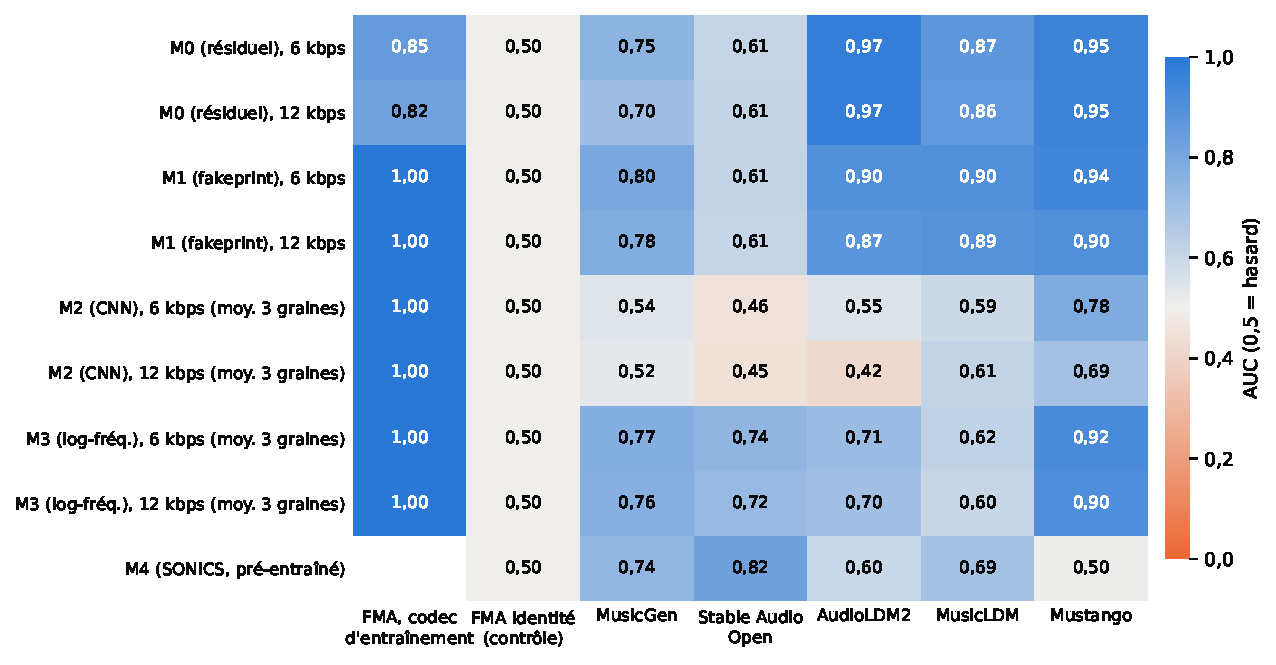
\includegraphics[width=\textwidth]{figures/fig_matrice_auc.pdf}
    \caption{Matrice de généralisation. AUC par détecteur et jeu de test ; pour M2 et M3, moyenne des trois
    graines. Orange : en dessous du hasard. La première colonne est le test sur le domaine d'entraînement,
    la deuxième le contrôle identité.}
    \label{fig:matrice}
\end{figure}

La corrélation de Spearman entre score de famille et AUC vaut $\rho = -0{,}348$, et son intervalle est
dégénéré ($[-0{,}348~;~-0{,}348]$). Ce n'est pas une erreur : le score de famille étant binaire (1 pour
MusicGen, 0 sinon), $\rho$ ne dépend que du rang de MusicGen parmi les dix AUC, et ce rang (7\textsuperscript{e}
et 8\textsuperscript{e}) ne change dans aucun tirage. Ce test est donc peu informatif par construction ; le
test confirmatoire sur l'écart est plus parlant. \textbf{H1 est réfutée.}

Pour H2, le test confirmatoire passe : l'AUC sur MusicGen dépasse 0,75 ($p$ corrigé $= 0{,}004$). Mais le
critère de réfutation est rempli par son autre branche : trois autres générateurs dépassent aussi 0,75.
\textbf{H2 est réfutée}\,---\,le transfert n'est pas « partiel et centré sur MusicGen », il est large et
indépendant de la famille du décodeur.

Les autres détecteurs nuancent le tableau. M3 est le seul à favoriser légèrement MusicGen : l'écart vaut
de $+0{,}014$ à $+0{,}037$ selon la graine et le débit, avec des intervalles qui excluent tous zéro
(annexe~\ref{app:graines}). L'effet est faible, et Mustango reste bien mieux détecté (0,92). M2, lui, est
instable : sur MusicGen, ses trois graines donnent 0,444, 0,611 et 0,576 à 6~kbit/s, et l'écart-type entre
graines atteint 0,25 sur Stable Audio Open à 12~kbit/s, bien plus que la largeur des intervalles bootstrap.
Une seule graine de M2 ne permettrait aucune conclusion.

\subsection{Ce que M1 a appris : un peigne à 75~Hz}
\label{sec:peigne}

Pourquoi le générateur de la même famille n'est-il pas mieux détecté ? Le pré-enregistrement prévoyait
d'examiner les empreintes moyennes et les poids appris (son §6.5) ; c'est ce qui répond le plus directement à la
question du titre. Pour chaque source, on calcule l'empreinte moyenne de 300 segments, on lui soustrait celle
des réels FMA, et on mesure le \emph{contraste de peigne} du profil obtenu : la valeur moyenne, en
écarts-types du profil, aux multiples d'un espacement $s$ donné. Un décodeur qui suréchantillonne à cadence
de trame fixe doit produire un contraste élevé quand $s$ est cette cadence (ou l'un de ses multiples).

\begin{figure}[h]
    \centering
    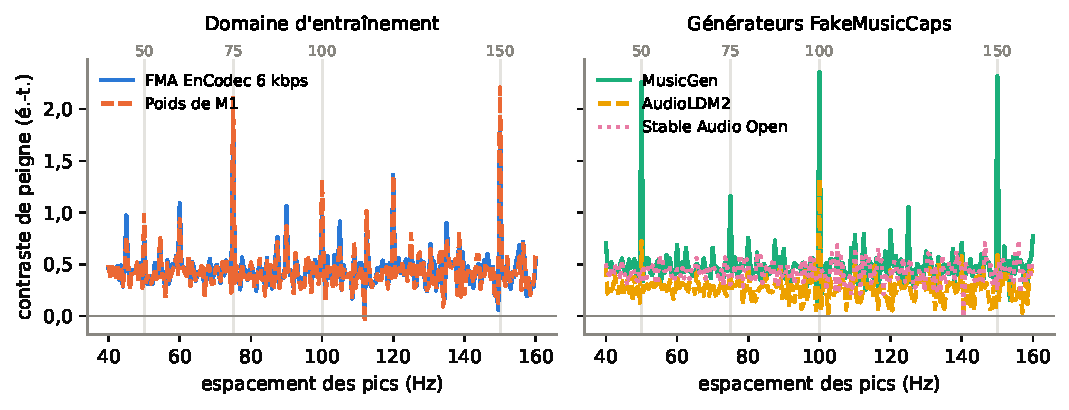
\includegraphics[width=\textwidth]{figures/fig_peigne.pdf}
    \caption{Contraste de peigne en fonction de l'espacement des pics. À gauche, l'empreinte des
    reconstructions EnCodec (moins celle des réels) et les poids de la régression logistique de M1 : tous
    deux culminent à 75 et 150~Hz. À droite, les générateurs : MusicGen culmine à 50, 100 et 150~Hz,
    AudioLDM2 montre un pic faible à 100~Hz, Stable Audio Open aucun. 300 segments par série ; mesure
    descriptive, sans intervalle de confiance.}
    \label{fig:peigne}
\end{figure}

Le résultat est sans ambiguïté (figure~\ref{fig:peigne}). \textbf{M1 a bien appris l'artefact du codec} :
ses douze plus grands poids tombent sur des multiples exacts de 75~Hz (2\,400, 3\,600, 4\,800, 6\,000,
7\,200~Hz\dots), la cadence d'EnCodec à 24~kHz, et le contraste de peigne de ses poids vaut 2,11 à 75~Hz
contre 0,97 à 50~Hz. Mais \textbf{MusicGen laisse un peigne espacé de 50~Hz} (contraste 2,26 à 50~Hz,
1,16 à 75~Hz), ce qui correspond à la cadence de 50~trames par seconde de son EnCodec à 32~kHz. Les deux
peignes ne coïncident qu'aux multiples de 150~Hz : M1 ne voit donc qu'une partie de l'artefact de MusicGen.
« Même famille de décodeur » ne veut pas dire « mêmes fréquences d'artefact ». Deux autres observations
complètent le tableau : Stable Audio Open ne laisse aucun peigne et c'est le générateur le plus difficile
pour tous les détecteurs ; AudioLDM2 n'a qu'un peigne faible, à 100~Hz, et il est pourtant parmi les mieux
détectés, ce qui renvoie au raccourci de la section suivante.

\subsection{Raccourcis de format (H3)}

\paragraph{Avant la chaîne : un raccourci total.} Prise seule comme score, chaque métadonnée de fichier
sépare les négatifs FMA des faux FakeMusicCaps (tableau~\ref{tab:meta}). Les fichiers FMA sont des MP3
stéréo de 30~s à 44,1 ou 48~kHz ; ceux de FakeMusicCaps des WAV mono de 10~s à 16~kHz. Un « détecteur »
qui lirait la durée du fichier aurait une AUC de 1. La chaîne commune efface ces différences ; la question
est ce qu'il en reste.

\begin{table}[h]
    \centering
    \small
    \begin{tabular}{lccc}
        \toprule
        Métadonnée & FMA (réels) & FakeMusicCaps (faux) & Séparabilité \\
        \midrule
        fréquence d'échantillonnage & 44,1 ou 48~kHz & 16~kHz & 1,000 \\
        débit & 128 à 320~kbit/s (MP3) & 512~kbit/s (WAV) & 1,000 \\
        durée & 30~s & 10 à 10,24~s & 1,000 \\
        canaux & mono ou stéréo & mono & 0,993 \\
        \bottomrule
    \end{tabular}
    \caption{Séparabilité ($\max(\mathrm{AUC}, 1-\mathrm{AUC})$) de chaque métadonnée prise seule comme
    score, identique pour les cinq générateurs. Sur les paires FMA, réel et faux héritent des métadonnées du
    même MP3 et la séparabilité vaut 0,5.}
    \label{tab:meta}
\end{table}

\paragraph{Après la chaîne : un raccourci résiduel.} M0, qui ne voit que des descripteurs triviaux calculés
après la chaîne, atteint 0,747 $[0{,}717~;~0{,}776]$ sur MusicGen ($p$ corrigé $= 0{,}004$), et ses
intervalles excluent 0,5 sur les cinq générateurs. \textbf{H3 n'est pas réfutée.} Le plus frappant est la
comparaison avec M1 (figure~\ref{fig:m0m1}, tableau~\ref{tab:m1m0}) : M0 fait \emph{mieux} que M1 sur
AudioLDM2 (0,971 contre 0,896) et sur Mustango à 12~kbit/s, et à peine moins bien ailleurs. Surtout, les
deux détecteurs s'accordent sur la difficulté des générateurs : Stable Audio Open puis MusicGen sont les
plus durs pour l'un comme pour l'autre, et les trois générateurs à VAE mel et vocodeur les plus faciles. Ce
que M1 « détecte » le mieux est donc aussi ce qui se distingue le plus de FMA par des propriétés de format.

\begin{figure}[h]
    \centering
    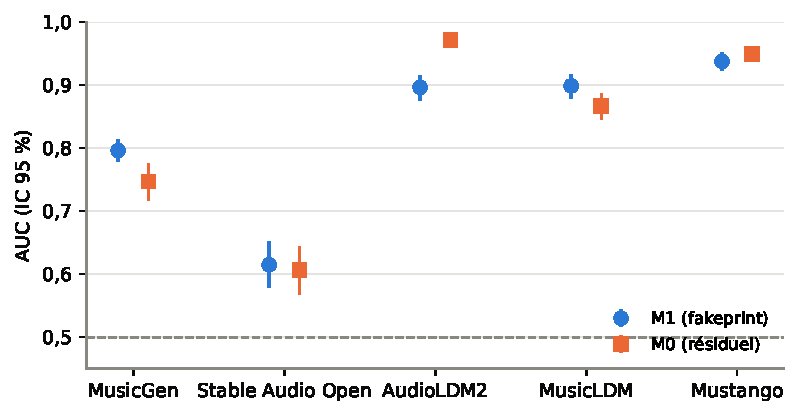
\includegraphics[width=0.78\textwidth]{figures/fig_m1_contre_m0.pdf}
    \caption{AUC de M1 (fakeprint) et de M0 (descripteurs triviaux) par générateur, détecteurs entraînés à
    6~kbit/s, IC~95~\% par bootstrap groupé. La ligne pointillée marque le hasard.}
    \label{fig:m0m1}
\end{figure}

\begin{table}[h]
    \centering
    \small
    \begin{tabular}{lcccc}
        \toprule
        & \multicolumn{2}{c}{6~kbit/s} & \multicolumn{2}{c}{12~kbit/s} \\
        \cmidrule(lr){2-3}\cmidrule(lr){4-5}
        Générateur & AUC M0 & M1 $-$ M0 [IC 95~\%] & AUC M0 & M1 $-$ M0 [IC 95~\%] \\
        \midrule
        MusicGen          & 0,747 & $+0{,}049$ $[+0{,}016~;~+0{,}089]$ & 0,701 & $+0{,}076$ $[+0{,}041~;~+0{,}117]$ \\
        Stable Audio Open & 0,607 & $+0{,}008$ $[-0{,}047~;~+0{,}067]$ & 0,611 & $-0{,}002$ $[-0{,}058~;~+0{,}061]$ \\
        AudioLDM2         & 0,971 & $-0{,}075$ $[-0{,}096~;~-0{,}053]$ & 0,969 & $-0{,}095$ $[-0{,}117~;~-0{,}070]$ \\
        MusicLDM          & 0,867 & $+0{,}032$ $[+0{,}005~;~+0{,}060]$ & 0,859 & $+0{,}032$ $[+0{,}005~;~+0{,}061]$ \\
        Mustango          & 0,950 & $-0{,}012$ $[-0{,}029~;~+0{,}005]$ & 0,950 & $-0{,}050$ $[-0{,}070~;~-0{,}030]$ \\
        \bottomrule
    \end{tabular}
    \caption{M0 et écart apparié M1 $-$ M0. M1 n'apporte un gain net que sur MusicGen et MusicLDM ; il est
    battu par M0 sur AudioLDM2, et sur Mustango à 12~kbit/s.}
    \label{tab:m1m0}
\end{table}

La seconde condition du critère de H3 (« M1/M2 ne chutent pas une fois le raccourci corrigé ») n'a pas été
mesurée : il aurait fallu identifier le descripteur responsable et l'effacer des deux bases. Elle n'intervient
pas dans le verdict, puisque la réfutation exigeait les deux conditions à la fois.

\subsection{Robustesse aux attaques (H4)}

La figure~\ref{fig:attaques} et le tableau~\ref{tab:attaques} montrent le résultat le plus net de l'étude.
Sous un ralentissement de 10~\%, M1 perd 0,162 ; sous une accélération de 10~\%, il perd 0,297 et tombe
exactement au hasard (0,499), avec un taux de détection de 0,3~\% au seuil fixé. M3 ne perd rien : son AUC
\emph{monte} de 0,010 et de 0,020. La différence appariée des deux variations vaut $-0{,}172$
$[-0{,}189~;~-0{,}154]$ sous $\times$0,9 et $-0{,}317$ $[-0{,}345~;~-0{,}287]$ sous $\times$1,1
($p$ corrigé $= 0{,}004$). Le critère de réfutation n'est pas atteint : \textbf{H4 n'est pas réfutée}.

\begin{figure}[h]
    \centering
    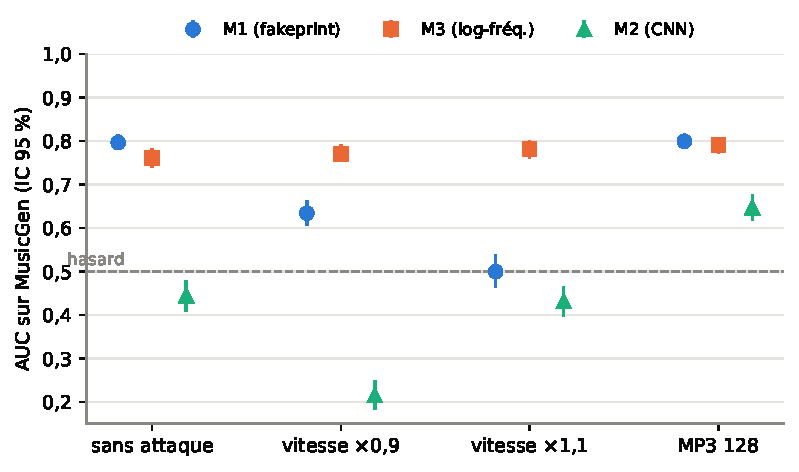
\includegraphics[width=0.78\textwidth]{figures/fig_attaques.pdf}
    \caption{AUC sur MusicGen sous attaque (détecteurs entraînés à 6~kbit/s ; M2 et M3 : graine~1).
    IC~95~\% par bootstrap groupé.}
    \label{fig:attaques}
\end{figure}

\begin{table}[h]
    \centering
    \small
    \begin{tabular}{llccc}
        \toprule
        Détecteur & Attaque & AUC & $\Delta$AUC [IC 95~\%] & TPR / FPR au seuil \\
        \midrule
        M1 & aucune      & 0,796 & ---                                    & 0,344 / 0,005 \\
           & vitesse $\times$0,9 & 0,634 & $-0{,}162$ $[-0{,}179~;~-0{,}144]$ & 0,197 / 0,007 \\
           & vitesse $\times$1,1 & 0,499 & $-0{,}297$ $[-0{,}324~;~-0{,}267]$ & 0,003 / 0,005 \\
           & MP3 128     & 0,799 & $+0{,}003$ $[+0{,}002~;~+0{,}004]$     & 0,364 / 0,005 \\
        \midrule
        M3 & aucune      & 0,761 & ---                                    & 0,379 / 0,016 \\
           & vitesse $\times$0,9 & 0,771 & $+0{,}010$ $[+0{,}003~;~+0{,}017]$ & 0,423 / 0,018 \\
           & vitesse $\times$1,1 & 0,781 & $+0{,}020$ $[+0{,}013~;~+0{,}028]$ & 0,395 / 0,023 \\
           & MP3 128     & 0,790 & $+0{,}029$ $[+0{,}025~;~+0{,}034]$     & 0,456 / 0,016 \\
        \midrule
        M2 & aucune      & 0,444 & ---                                    & 0,001 / 0,014 \\
           & vitesse $\times$0,9 & 0,215 & $-0{,}229$ $[-0{,}272~;~-0{,}185]$ & 0,047 / 0,325 \\
           & vitesse $\times$1,1 & 0,431 & $-0{,}013$ $[-0{,}065~;~+0{,}037]$ & 0,098 / 0,195 \\
           & MP3 128     & 0,646 & $+0{,}202$ $[+0{,}187~;~+0{,}219]$     & 0,037 / 0,020 \\
        \bottomrule
    \end{tabular}
    \caption{Attaques sur le test MusicGen. $\Delta$AUC apparié (attaque $-$ sans attaque) ; seuil fixé sur
    la validation propre, jamais réajusté.}
    \label{tab:attaques}
\end{table}

Deux prédictions accessoires sont en revanche démenties. Le MP3 à 128~kbit/s ne fait chuter ni M1 ni M3
(prédit : $-0{,}05$ à $-0{,}15$ pour les deux), et M3 en sort même plus robuste que M1 ($-0{,}026$
$[-0{,}031~;~-0{,}022]$ en faveur de M3). M2 réagit de façon erratique : sous le hasard sans attaque, il
s'inverse davantage sous ralentissement (0,215, et son taux de faux positifs passe de 1,4 à 32,5~\%) et
remonte à 0,646 sous MP3.

\subsection{Synthèse des tests confirmatoires}

\begin{table}[h]
    \centering
    \small
    \begin{tabularx}{\textwidth}{lYccc}
        \toprule
        & Test confirmatoire & Valeur [IC 95~\%] & $p$ / $p$ Holm & Verdict selon le critère \\
        \midrule
        H1 & AUC(MusicGen) $-$ moyenne des autres $> 0$ & $-0{,}041$ $[-0{,}052~;~-0{,}029]$ & 1,000 / 1,000 & réfutée \\
        H2 & AUC(MusicGen) $> 0{,}75$ & 0,796 $[0{,}779~;~0{,}814]$ & 0,001 / 0,004 & réfutée \\
        H3 & AUC(M0 $\to$ MusicGen) $> 0{,}5$ & 0,747 $[0{,}717~;~0{,}776]$ & 0,001 / 0,004 & non réfutée \\
        H4 & $\Delta$AUC(M1) $-$ $\Delta$AUC(M3) $< 0$, $\times$1,1 & $-0{,}317$ $[-0{,}345~;~-0{,}287]$ & 0,001 / 0,004 & non réfutée \\
        \bottomrule
    \end{tabularx}
    \caption{Tests confirmatoires (M1 et M0 entraînés à 6~kbit/s ; M3 graine~1), corrigés ensemble par Holm.
    Un test significatif ne signifie pas une hypothèse confirmée : H2 passe son test mais est réfutée par la
    seconde branche de son critère.}
    \label{tab:confirmatoires}
\end{table}

\subsection{Analyses secondaires}

\paragraph{Une AUC correcte cache un seuil inutilisable.} Le seuil fixé à 1~\% de faux positifs sur FMA
reste valable pour les réels (le FPR observé est de 0,5~\% pour M1), puisqu'ils viennent du même domaine.
Mais il ne se transfère pas aux faux : pour M1, le taux de détection n'est que de 34~\% sur MusicGen, 11~\%
sur AudioLDM2, 10~\% sur MusicLDM, 15~\% sur Mustango et 1,7~\% sur Stable Audio Open, malgré des AUC de
0,8 à 0,94. Les scores des faux FakeMusicCaps sont bien ordonnés mais beaucoup plus bas que ceux des faux
d'entraînement, et l'erreur de calibration est forte (ECE de 0,71 à 0,85). En pratique, un tel détecteur
déployé tel quel manquerait la plupart des extraits générés.

\paragraph{Le détecteur externe.} M4 (SONICS) obtient 0,820 sur Stable Audio Open, 0,735 sur MusicGen, mais
0,601 sur AudioLDM2 et 0,505 sur Mustango : son profil est presque l'inverse de celui de M1 et de M0, ce qui
est cohérent avec un détecteur qui a appris d'autres artefacts, ou d'autres raccourcis, sur d'autres données.

\paragraph{Faux positifs par genre.} Au seuil fixé, le taux de faux positifs reste faible dans tous les
genres : au plus 2~\% pour M1, au plus 6,1~\% pour M3 (« Experimental », 6 segments sur 98) et 8,3~\% dans
le pire cas (M2, graine~3, « Instrumental », 3 segments sur 36) (annexe~\ref{app:genre}). Avec 36 à 136
segments par genre, ces mesures sont trop peu nombreuses pour exclure un biais modéré.

\paragraph{Les pires erreurs.} Les vingt réels que M1 juge les plus suspects viennent de 17 pistes, surtout
« Experimental » (5) et « Electronic » (4). Les faux MusicGen les plus manqués reçoivent un score
quasi nul : le détecteur ne doute pas, il se trompe avec assurance, ce qui est le symptôme attendu d'une
décision fondée sur autre chose que l'artefact.

% =====================================================================================================
\section{Discussion}
\label{sec:discussion}

\paragraph{Ce que voit le détecteur.} Sur son propre domaine, le détecteur voit bien l'artefact du codec :
AUC de 1 contre la reconstruction EnCodec, 0,5 contre la reconstruction identité, sans fuite de la chaîne,
et des poids alignés sur les multiples de 75~Hz.
Hors de ce domaine, trois observations convergent vers une autre lecture. Les métadonnées des deux bases
les séparent parfaitement ; un détecteur de raccourcis qui ignore tout du codec rivalise avec le meilleur
détecteur appris ; et les générateurs que M1 détecte le mieux sont ceux que ce détecteur trivial
détecte le mieux, pas ceux de la famille d'EnCodec. Sur ce protocole, une AUC élevée sur \texttt{fmc:<générateur>} mesure donc surtout ce qui
distingue un fichier FakeMusicCaps d'un fichier FMA. Ce n'est pas un défaut des détecteurs : c'est ce que
le test leur permet d'apprendre, faute d'extraits réels MusicCaps à opposer aux faux.

\paragraph{Pourquoi MusicGen n'est pas plus facile.} H1 supposait que « même famille » voulait dire
« mêmes artefacts ». La section~\ref{sec:peigne} montre que c'est faux à un niveau très concret : le
détecteur a appris un peigne à 75~Hz, la cadence de l'EnCodec d'entraînement, et MusicGen laisse un peigne à
50~Hz, la cadence de son propre EnCodec. C'est ce que prédit l'explication des artefacts par la cadence des
trames \cite{afchar2025fourier}. Le score de famille du pré-enregistrement était donc un mauvais prédicteur,
indépendamment du raccourci : la variable pertinente est la cadence du décodeur, pas sa famille.
L'expérience « oracle » prévue, qui entraîne sur l'EnCodec exact de MusicGen, testerait directement cette
lecture ; elle n'a pas été réalisée.

\paragraph{Ce que H4 établit, et ce qu'il n'établit pas.} H4 est la conclusion la plus solide : la
comparaison porte sur les mêmes segments, avec le même tirage bootstrap, et l'écart est massif. Le
mécanisme attendu est clair : un changement de vitesse de facteur $a$ multiplie toutes les fréquences par
$a$, de sorte que les pics espacés de 75~Hz le sont désormais de 82,5~Hz sous $\times$1,1 et ne tombent plus
sur les poids linéaires de M1 ; en log-fréquence, ce n'est qu'une translation, absorbée par le maximum de
la corrélation croisée de M3. Deux réserves s'imposent toutefois. D'abord, M3 a été entraîné \emph{avec}
une augmentation par changement de vitesse entre $\times$0,7 et $\times$1,4, qui couvre les attaques
testées : sa robustesse peut venir de l'architecture, de l'augmentation, ou des deux, et il faudrait
entraîner M3 sans augmentation (ou M1 avec) pour le savoir. Ensuite, l'AUC de base sur MusicGen contient
une part de raccourci ; H4 montre que la décision de M1 est fragile, pas exactement ce qu'elle perd.

\paragraph{Des attaques qui améliorent.} M3 gagne de 0,010 à 0,029 sous les trois attaques, et M2 gagne
0,202 sous MP3. Une attaque qui ne ferait qu'effacer des artefacts devrait faire baisser l'AUC. Une
explication possible, non testée ici, est que l'attaque transforme différemment les deux bases (MP3
d'origine contre WAV à 16~kHz) et accentue ce qui les distingue. C'est un argument de plus pour lire les
AUC FakeMusicCaps comme des mesures d'écart entre bases.

\paragraph{Mes prédictions.} Sur dix-sept fourchettes chiffrées avant l'expérience, trois contiennent la
valeur observée (annexe~\ref{app:predictions}). Les erreurs ne sont pas aléatoires : j'avais prédit des
AUC de 0,55 à 0,65 pour M1 sur AudioLDM2, MusicLDM et Mustango, en raisonnant sur les familles de
décodeurs, et j'observe 0,87 à 0,94 ; le raccourci, que je n'avais pas chiffré, explique précisément cet
écart. Le pré-enregistrement a joué son rôle : sans lui, il aurait été tentant de lire ces AUC élevées
comme une généralisation réussie.

\paragraph{Limites.} Les principales sont les suivantes.
\begin{itemize}
    \item Pas d'extraits réels MusicCaps : le contraste FakeMusicCaps mélange génération et domaine. C'est
    la limite qui conditionne toutes les autres lectures.
    \item Un seul codec d'entraînement (EnCodec 24~kHz, deux débits) et 2\,000 pistes ; la phase complète
    prévue (8\,000 pistes, DAC) n'a pas été réalisée.
    \item Attaques mesurées sur un seul générateur (MusicGen), une seule graine de M3, et pas sur le domaine
    d'entraînement, où l'effet de la vitesse sur l'artefact serait mesuré sans raccourci.
    \item La graine 3 de M2 et M3 (et M3 à 12~kbit/s, graine~2) a été entraînée dans un autre environnement
    logiciel et matériel que les autres (annexe~\ref{app:repro}) ; l'écart entre graines inclut donc aussi
    cet écart d'environnement.
\end{itemize}

% =====================================================================================================
\section{Conclusion et perspectives}

Un détecteur entraîné à reconnaître la reconstruction de musique réelle par EnCodec voit très bien
l'artefact du codec sur son propre domaine. Testé sur des générateurs inconnus, il obtient des AUC
souvent élevées, mais sans lien avec la famille de décodeur, et un détecteur qui ne voit que des
descripteurs de format fait aussi bien : ces AUC mesurent surtout la différence entre deux bases de
données. La robustesse comparée est en revanche un résultat net : un fakeprint en log-fréquence, appris
avec augmentation, résiste aux changements de vitesse qui annulent le fakeprint linéaire.

Les suites les plus utiles découlent directement des limites :
\begin{enumerate}
    \item opposer les faux à des réels \emph{du même domaine} (extraits MusicCaps réels, ou réels et faux
    issus d'une même chaîne de production), seule façon de mesurer la généralisation sans raccourci ;
    \item réaliser l'oracle MusicGen (entraînement sur l'EnCodec 32~kHz de MusicGen) pour tester si
    l'artefact dépend de la cadence du codec plutôt que de sa famille ;
    \item séparer l'architecture et l'augmentation dans la robustesse de M3, et mesurer les attaques sur le
    domaine d'entraînement ;
    \item recalibrer les scores (mise à l'échelle par température) et rapporter les taux de détection à
    FPR fixé, plus proches d'un usage réel que l'AUC.
\end{enumerate}

\printbibliography[heading=bibintoc, title={Références}]

% =====================================================================================================
\newpage
\appendix

\section{Écarts au pré-enregistrement}
\label{app:ecarts}

\begin{itemize}
    \item \textbf{Phase complète non réalisée} (8\,000 pistes, DAC), ni l'oracle MusicGen, ni l'oracle
    Stable Audio Open, ni le test d'écoute. H1 a été testée sur 5 générateurs $\times$ 2 débits, ce que son
    propre critère prévoit.
    \item \textbf{Analyse d'erreurs (§6.5) partielle.} Les empreintes moyennes et les poids de M1 sont
    analysés (section~\ref{sec:peigne}), avec une mesure de contraste de peigne définie après coup ; les
    filtres de M3 et l'écoute des vingt pires erreurs ne le sont pas.
    \item \textbf{H1 : Spearman dégénéré.} Avec un score de famille binaire, $\rho$ ne dépend que du rang de
    MusicGen ; l'intervalle est réduit à un point.
    \item \textbf{H3 : seconde condition non mesurée} (effet d'une correction du raccourci sur M1/M2).
    \item \textbf{M0 « brut » remplacé par une mesure directe.} Entraîné sur les paires FMA, un détecteur de
    métadonnées n'apprendrait rien (réel et faux héritent du même MP3). La séparabilité de chaque
    métadonnée est mesurée directement sur les tests FakeMusicCaps (tableau~\ref{tab:meta}).
    \item \textbf{Attaques :} seules les trois attaques pré-enregistrées sont mesurées, sur MusicGen, avec
    la graine~1 de M2 et M3.
    \item \textbf{Holm :} le pré-enregistrement annonce une correction « sur les 5 comparaisons
    confirmatoires (une par hypothèse) » alors qu'il y a quatre hypothèses ; la correction porte ici sur
    les quatre tests confirmatoires. Pour H2, une correction de Holm sur les cinq générateurs est
    aussi calculée (elle ne change rien au verdict).
    \item \textbf{Réévaluation de M0 à 12~kbit/s.} Une première évaluation a été faite avec une version
    de scikit-learn différente de celle qui avait enregistré le modèle ; elle a été jetée et refaite avec
    la bonne version (annexe~\ref{app:repro}).
\end{itemize}

\section{Prédictions et observations}
\label{app:predictions}

\begin{table}[H]
    \centering
    \small
    \begin{tabular}{llccc}
        \toprule
        Détecteur & Générateur ou attaque & Prédit & Observé & Dans la fourchette \\
        \midrule
        M1 & MusicGen          & 0,80 -- 0,90 & 0,796 & non (juste en dessous) \\
        M1 & Stable Audio Open & 0,55 -- 0,65 & 0,615 & oui \\
        M1 & AudioLDM2         & 0,55 -- 0,65 & 0,896 & non \\
        M1 & MusicLDM          & 0,55 -- 0,65 & 0,899 & non \\
        M1 & Mustango          & 0,55 -- 0,70 & 0,938 & non \\
        M0 & MusicGen          & 0,60 -- 0,70 & 0,747 & non \\
        M4 & MusicGen          & 0,75 -- 0,85 & 0,735 & non \\
        M4 & Stable Audio Open & 0,65 -- 0,75 & 0,820 & non \\
        M4 & AudioLDM2         & 0,65 -- 0,75 & 0,601 & non \\
        M4 & MusicLDM          & 0,65 -- 0,75 & 0,691 & oui \\
        M4 & Mustango          & 0,60 -- 0,70 & 0,505 & non \\
        \midrule
        M1 & $\Delta$ vitesse $\times$0,9 & $-0{,}25$ -- $-0{,}15$ & $-0{,}162$ & oui \\
        M1 & $\Delta$ vitesse $\times$1,1 & $-0{,}25$ -- $-0{,}15$ & $-0{,}297$ & non (chute plus forte) \\
        M1 & $\Delta$ MP3 128             & $-0{,}15$ -- $-0{,}05$ & $+0{,}003$ & non \\
        M3 & $\Delta$ vitesse $\times$0,9 & $-0{,}08$ -- $-0{,}02$ & $+0{,}010$ & non (meilleur) \\
        M3 & $\Delta$ vitesse $\times$1,1 & $-0{,}08$ -- $-0{,}02$ & $+0{,}020$ & non (meilleur) \\
        M3 & $\Delta$ MP3 128             & $-0{,}15$ -- $-0{,}05$ & $+0{,}029$ & non \\
        \bottomrule
    \end{tabular}
    \caption{Les dix-sept prédictions chiffrées du pré-enregistrement (détecteurs entraînés à 6~kbit/s).}
\end{table}

\section{Résultats par graine}
\label{app:graines}

\begin{table}[H]
    \centering
    \footnotesize
    \setlength{\tabcolsep}{4.5pt}
    \begin{tabular}{llccccccc}
        \toprule
        Détect. & Débit & Graine & MusicGen & S.\,A.\,Open & AudioLDM2 & MusicLDM & Mustango & MG $-$ autres \\
        \midrule
        M2 & 6  & 1 & 0,444 & 0,374 & 0,363 & 0,469 & 0,669 & $-0{,}025$ \\
        M2 & 6  & 2 & 0,611 & 0,498 & 0,606 & 0,626 & 0,790 & $-0{,}019$ \\
        M2 & 6  & 3 & 0,576 & 0,493 & 0,682 & 0,678 & 0,894 & $-0{,}111$ \\
        M2 & 12 & 1 & 0,454 & 0,448 & 0,316 & 0,534 & 0,721 & $-0{,}051$ \\
        M2 & 12 & 2 & 0,695 & 0,697 & 0,603 & 0,735 & 0,764 & $-0{,}004$ \\
        M2 & 12 & 3 & 0,421 & 0,199 & 0,331 & 0,576 & 0,585 & $-0{,}002$ \\
        \midrule
        M3 & 6  & 1 & 0,761 & 0,746 & 0,711 & 0,616 & 0,917 & $+0{,}014$ \\
        M3 & 6  & 2 & 0,767 & 0,744 & 0,715 & 0,620 & 0,923 & $+0{,}016$ \\
        M3 & 6  & 3 & 0,770 & 0,736 & 0,712 & 0,619 & 0,925 & $+0{,}022$ \\
        M3 & 12 & 1 & 0,762 & 0,722 & 0,697 & 0,602 & 0,904 & $+0{,}031$ \\
        M3 & 12 & 2 & 0,767 & 0,726 & 0,700 & 0,604 & 0,910 & $+0{,}032$ \\
        M3 & 12 & 3 & 0,765 & 0,714 & 0,691 & 0,604 & 0,900 & $+0{,}037$ \\
        \bottomrule
    \end{tabular}
    \caption{AUC par graine sur FakeMusicCaps (débit d'entraînement en kbit/s). Dernière colonne : écart
    MusicGen $-$ moyenne des quatre autres ; pour M3, les six intervalles excluent zéro. Sur leur domaine,
    toutes les graines atteignent 0,996 à 0,999.}
\end{table}

\section{Faux positifs par genre}
\label{app:genre}

\begin{table}[H]
    \centering
    \small
    \begin{tabular}{lccccccccc}
        \toprule
        Genre & $n$ & M0 & M1 & M2 g1 & M2 g2 & M2 g3 & M3 g1 & M3 g2 & M3 g3 \\
        \midrule
        Electronic    & 94  & 0,000 & 0,000 & 0,021 & 0,011 & 0,011 & 0,000 & 0,000 & 0,000 \\
        Experimental  & 98  & 0,031 & 0,020 & 0,020 & 0,031 & 0,010 & 0,061 & 0,061 & 0,041 \\
        Folk          & 118 & 0,000 & 0,000 & 0,008 & 0,000 & 0,000 & 0,008 & 0,008 & 0,008 \\
        Hip-Hop       & 78  & 0,013 & 0,000 & 0,013 & 0,000 & 0,026 & 0,000 & 0,000 & 0,000 \\
        Instrumental  & 36  & 0,028 & 0,000 & 0,000 & 0,000 & 0,083 & 0,028 & 0,028 & 0,028 \\
        International & 136 & 0,022 & 0,007 & 0,007 & 0,007 & 0,007 & 0,007 & 0,007 & 0,007 \\
        Pop           & 88  & 0,000 & 0,011 & 0,000 & 0,011 & 0,000 & 0,034 & 0,034 & 0,034 \\
        Rock          & 84  & 0,000 & 0,000 & 0,036 & 0,024 & 0,000 & 0,000 & 0,000 & 0,000 \\
        \bottomrule
    \end{tabular}
    \caption{Taux de faux positifs par genre sur les 732 segments réels du test FMA, au seuil fixé sur la
    validation (cible : 1~\%). $n$ : nombre de segments. Détecteurs entraînés à 6~kbit/s.}
\end{table}

\section{Reproductibilité et calcul}
\label{app:repro}

\paragraph{Code.} Le dépôt \texttt{musicdetect} contient la chaîne, les détecteurs, l'évaluation et le
module \texttt{musicdetect.analysis}, qui recalcule toutes les statistiques de ce rapport à partir des scores
par segment (\texttt{results/<tag>/scores/}) :
\begin{center}
\footnotesize\texttt{python -m musicdetect.analysis -{}-results results -{}-fma-index \dots{} -{}-fmc-index \dots{} -{}-out \dots}
\end{center}
Les figures et tableaux en sont tirés sans retouche ; le bootstrap utilise la graine 0. La figure du
peigne (figure~\ref{fig:peigne}) vient du module \texttt{musicdetect.peigne}, qui relit le modèle M1 et
300 segments par source.

\paragraph{Déroulement.} M0, M1 et les graines 1 et 2 de M2 et M3 (sauf M3 à 12~kbit/s, graine~2) ont été
entraînés sur un ordinateur personnel, sur CPU (Python 3.13, scikit-learn 1.9.1, PyTorch 2.15, NumPy 2.5).
Des interruptions, dont un redémarrage par Windows Update, ont conduit à terminer sur Kaggle, en trois
sessions : une sur GPU T4 (3,8~h : graine~3 de M2 et M3 et M3 à 12~kbit/s graine~2, premières attaques de M2
et M3), deux sur CPU (0,8~h : réévaluation de M0 et M1 à 12~kbit/s et attaques de M1 ; 8,3~h : attaques des
trois détecteurs refaites avec enregistrement des scores par segment). L'image Kaggle fournissait Python 3.13, NumPy 2.1, SciPy 1.16 et PyTorch 2.11 ;
scikit-learn y a été imposé en version 1.9.1, car M0 et M1 sont enregistrés par sérialisation
(\emph{pickle}) et une autre version faisait échouer M1 ou rendait les scores de M0 douteux.

\paragraph{Calcul et stockage.} Les attaques dominent le coût : l'aller-retour MP3 lance un encodeur par
segment. Sur CPU, une grille de trois attaques sur MusicGen a pris 70~min pour M1, 4,6~h pour M3 et 2,5~h
pour M2. Les segments occupent environ 13~Go ; modèles, scores et résultats environ 25~Mo.

\section{Glossaire}

\begin{description}
    \item[AUC] aire sous la courbe ROC ; probabilité qu'un faux tiré au hasard reçoive un score plus élevé
    qu'un réel tiré au hasard. 0,5 : hasard ; 1 : séparation parfaite ; sous 0,5 : décision inversée.
    \item[Bootstrap groupé] rééchantillonnage avec remise de groupes entiers (artistes, légendes) plutôt que
    de segments, pour respecter leur dépendance.
    \item[Codec neuronal] réseau qui compresse le signal en jetons discrets et le reconstruit ; la
    quantification vectorielle résiduelle empile plusieurs dictionnaires, chacun codant l'erreur du précédent.
    \item[ECE] erreur de calibration : écart moyen entre le score annoncé et la fréquence réelle des faux.
    \item[Fakeprint] résidu du spectre moyen au-dessus de son enveloppe inférieure ; il isole les pics fins
    et réguliers laissés par un décodeur.
    \item[FPR, TPR] taux de faux positifs (réels déclarés faux) et taux de détection (faux déclarés faux) à
    un seuil donné.
    \item[Holm] correction des tests multiples : les $m$ valeurs $p$ triées sont comparées à
    $\alpha/m, \alpha/(m-1), \dots$, ce qui contrôle le risque de faux positif sur l'ensemble des tests.
    \item[Raccourci] indice qui sépare les classes dans les données d'étude sans être la propriété visée
    (ici : format, bande passante, durée).
    \item[Test apparié] comparaison de deux mesures sur les mêmes exemples, qui élimine la variabilité due
    aux exemples eux-mêmes.
\end{description}

\end{document}
